
%% bare_conf.tex
%% V1.3
%% 2007/01/11
%% by Michael Shell
%% See:
%% http://www.michaelshell.org/
%% for current contact information.
%%
%% This is a skeleton file demonstrating the use of IEEEtran.cls
%% (requires IEEEtran.cls version 1.7 or later) with an IEEE conference paper.
%%
%% Support sites:
%% http://www.michaelshell.org/tex/ieeetran/
%% http://www.ctan.org/tex-archive/macros/latex/contrib/IEEEtran/
%% and
%% http://www.ieee.org/

\documentclass[10pt, conference]{IEEEtran}

\usepackage{booktabs}
\usepackage{cite}
\usepackage{color}
\usepackage{enumitem}
\usepackage{float}
\usepackage[utf8]{inputenc}
\usepackage{tikz}
\usepackage{multicol}
\usepackage{multirow}
\usepackage{subcaption}
\usepackage[skip=0pt]{caption}
\usepackage{url}
\usepackage{rotating}

\makeatletter
\setlength{\@fptop}{0pt}
\makeatother

\newif\ifComments

% To turn comments OFF simply comment out the \Commentstrue line
\Commentstrue

\ifComments
\newcommand{\luiz}[1]{\noindent\textcolor{orange}{LUIZ: {#1}}}
\newcommand{\mario}[1]{\noindent\textcolor{green}{MARIO: {#1}}}
\newcommand{\rem}[1]{\noindent\textcolor{magenta}{REMOVED: {#1}}}
\newcommand{\new}[1]{\noindent\textcolor{blue}{NEW: {#1}}}
\else
\newcommand{\luiz}[1]{}
\newcommand{\mario}[1]{}
\newcommand{\rem}[1]{}
\newcommand{\new}[1]{#1}
\fi

% correct bad hyphenation here
\hyphenation{}

\begin{document}

\title{Machine Learning Based Prediction of CR Severity Level in FLOSS: Experimental Results
}

\author{
	\IEEEauthorblockN{Luiz Alberto Ferreira Gomes\\\texttt{gomes.luiz@ic.unicamp.br}}
	\IEEEauthorblockA{Institute of Computing, University of Campinas, Brazil.}
	\and
	\IEEEauthorblockN{Mario Lucio Cortes\\\texttt{cortes@ic.unicamp.br}}
	\IEEEauthorblockA{Institute of Computing, University of Campinas, Brazil}
}
\maketitle
\begin{abstract}
In the context of Change Request (CR) systems, the severity level of a change request is considered a critical variable when planning software maintenance activities, indicating how soon a CR needs to be addressed. However, the severity level assignment remains primarily a manual process, mostly depending on the experience and expertise of the person who has reported the CR. This paper presents preliminary findings on the prediction of CR severity level by analyzing its long description, using text mining techniques and Machine Learning (ML) algorithms. We have collected CRs from three FLOSS projects (imbalanced) repositories: Cassandra, Hadoop and Spark. Ours results were better than those published in the literature in terms of F-measure performance for two research questions (using Random Forest) and similar for the third research question. However, subsequent analyses based on the Friedman test have demonstrated that data used in experiments haven't permitted us to say with enough confidence level that Random Forest is better than the others ML algorithms. We have also shown that the use classical ML measurements available in the literature may not help deciding whether a ML approach will bring any benefit to the user, and have proposed an alternative measuring approach to address this issue.
\end{abstract}


\begin{IEEEkeywords}
software maintenance; change request systems; text mining; machine learning; software repositories.
\end{IEEEkeywords}

\IEEEpeerreviewmaketitle
\section{Introduction}
Change Request (CR) systems have played a major role in maintenance process in many software development settings, both in Closed Source Software (CSS) and in Open Source Software (OSS) scenarios. This is especially true in OSS, which is characterized by the existence of many of users and developers with different levels of expertise spread out around the world, who might create or be responsible for dealing with several CRs\cite{Cavalcanti2014}.

A user interacts with a CR system often through a simple mechanism called CR form. This form enables him to request changes, to report bugs or to ask for support in a software product\cite{Sommerville2010}. Initially, he or she should inform a short description, a long description, a type (e.g. bug, new feature, enhancement, and task) and an associated severity level (e.g. blocker, critical, major, minor and trivial). Subsequently, a development team member will review this request and, case it is not refused for some reason (e.g. request duplication), he or she will complete the information in CR form, indicating, for example, its priority and assigning the person responsible for the CR. 

The severity level information is recognized as a critical variable in the equation to estimate a prioritization of CRs \cite{Tian2012}. It defines how soon the CR needs to be addressed\cite{Lamkanfi2010}. However, the severity level assignment remains mostly a manual process which relies only on the experience and expertise of the person who has opened the CR \cite{Cavalcanti2014, Tian2012, Lamkanfi2010}. Consequently, it is a process with high degree of subjectivity, and it may be quite error-prone. 

The number of CRs in large and medium software OSS projects is frequently very large\cite{Lamkanfi2011}: Eclipse project received over 2.764 requests and GNOME project received over 3.263 requests between 01$/$10$/$2009 and 01$/$01$/$2010. Severity level shifts throughout CR lifecycle may have an adverse effect on planning of maintenance activities. For example, the maintenance team could be assigned to address less significant CRs before  most important ones. There has been reports \cite{Tian2015} of efforts to implement intelligent software assistants to help developers and maintenance personnel in defining more accurately the field values in a CR form. Currently, Machine Learning techniques have become a popular method to address this issue and there are quite a few publications in this area in the literature \cite{Cavalcanti2014}. 

Machine Learning (ML) techniques have been successfully applied in solving real problems in many areas of knowledge, including those related to CR systems, such as duplication and assignment of CR\cite{Cavalcanti2014}. However, the accuracy of ML algorithms may be affected by imbalanced datasets \cite{Chawla2009} \textemdash  a recurring critical problem in CR repositories\cite{Tian2015}. For example, more than 60\% of CRs may have a ``major'' severity level. In addition to this problem, most publications are still focused in predicting the severity level of CRs and none of them have been implemented into popular tools like as Bugzilla, Jira and Redmine.\cite{Cavalcanti2014}. Furthermore, many have used proprietary and/or not public ML algorithms. Therefore, there is still a clear need of advances in this knowledge area, specially broadening the reach of research questions and including more popular and open OSS and ML algorithms.

In this context, the general purpose of our research is to develop an intelligent ML based assistant to help developers and maintenance personnel in the OSS maintenance activities. In this current article, our specific goals are: 

\begin{enumerate}[label=\textbf{G$_\arabic*$}.]
  \item Evaluate the performance of traditional ML algorithms in the prediction of CR severity level and identify a suitable algorithm to perform such prediction in a scenario where imbalanced data is natural;
  \item Apply statistical tests to confirm if a ML algorithm is better than the others.  
  \item Analyze whether ML algorithms outperforms a human user in predicting CR severity level and propose new approaches, accordingly. 
\end{enumerate}

To meet these goals, this research works with the following research questions, regarding CR severity level during its lifecycle:

\begin{enumerate}[label=\textbf{RQ$_\arabic*$}.]
  \item \textit{Will the CR severity level change?}
  \item \textit{Will the CR severity level increase, decrease or remain the same}? 
  \item \textit{What is the prediction for the final CR severity level?}
  \item \textit{How ML predictions compare to user prediction?} 
\end{enumerate}

The first three research questions are related to goals 1 and 2, and the last one is related to goal 3

The contributions of our research are:
\begin{itemize}
  \item Analyze the performance of three popular ML algorithms as multi category classifiers in imbalanced datasets extracted from three FLOSS repositories. 
  \item Run statistical tests on experimental results and demonstrate that, under these conditions, it is not possible to guarantee that an algorithm is better than others with appropriate confidence level.
  \item Analyze how well an automated ML based predictor performs with respect to a user prediction and propose new measurement approach.
\end{itemize}

The article is organized as follows. Section \ref{sec:relatedwork} presents related work that are relevant to our research. Section \ref{sec:background} provides the information background about CR systems, text mining and machine learning techniques necessary to understand our approach. Section \ref{sec:experiment} describes our work. Section \ref{sec:discussion} presents final findings and discussion. Finally, Section \ref{sec:conclusion} present  conclusions and  future work.


\section{Related Work}\label{sec:relatedwork} 

This section presents relevant articles in mining open system repositories, aiming at extracting data and using ML techniques to predict several maintenance properties. 

Menzies and Marcus\cite{Menzies2008} have developed a method, named SEVERIS (SEVERity ISsue assessment), for evaluating the severity of CRs. SEVERIS is based on established data and text mining techniques. The method was applied to predict CR severity level in five projects managed by the Project and Issue Tracking System (PITS), an issue tracker system used by NASA (Stratified F-measures by severity level in the range: (2) 78\%-86\%; (3) 68\%-98\%; (4) 86\%-92\%).


Lamkanfi et al.\cite{Lamkanfi2010} have developed an approach to predict if severity of bug report is non-severe (severity levels: 1 or 2) or severe (severity levels: 4 or 5) based on text mining algorithms (tokenization, stop word removal, stemming) and on the Naïve Bayes machine learning algorithm. They have validated their approach with data from three open source project (Mozilla, Eclipse, and GNOME). The article reports that a training set with approximately 500 CRs per severity level is sufficient to make predictions with reasonable accuracy (precision and recall in the range 0.65-0.75 with Mozilla and Eclipse; 0.70-0.85 with GNOME).

Valdivia et al.\cite{ValdiviaGarcia2014} have characterized blocking bugs in six open source projects and proposed a model to predict them. Their model was composed of 14 distinct factors or features (e.g. the textual description, location the bug is found in and the people involved with the bug). Based on these factors they have built decision trees for each project to predict whether a bug will be a blocking bug or not (F-measures in the range 15-42\%).

Tian et al.\cite{Tian2012} have develop a method to predict the severity level of new CRs based on similar CRs reported in the past. The comparison between old and new CRs was implemented by the BM25 similarity function. This method was applied to Mozilla, Eclipse and OpenOffice projects over more than 250,000 CR extracted from Bugzilla (F-measure in the range 13.9-65.3\% for Mozilla; 8.6-58\% for Eclipse; and 12.3-74\% for OpenOffice). 



\section{Terminology and Background}\label{sec:background} 
This section presents an overview on general concepts necessary to understand this research area, namely Bug Tracking Systems, Machine Learning (algorithms, feature selection methods, evaluation measures, and sampling methods), and Statistical Tests. More specific concepts will be detailed as they are cited in the document.

\subsection{Bug Tracking System (BTS)}

BTS\cite{Lamkanfi:2010} is a software application that keeps the record and tracks information about change requests, bug fixes, and technical support that could occur during the software lifecycle. Usually, while reporting a bug in a BTS, a user is asked to provide information about the bug by filling out a form, typically called bug report form. 

\subsubsection{Bug Report}
Although there is no agreement on the terminology or the amount of information that users must provide to fill a typical bug report (illustrated in Figure \ref{fig:bug-report-example}, the example refers to a bug report extracted from Bugzilla of Eclipse project.), they often describe their needs in popular BTS (e.g., Bugzilla, Jira, and Redmine)\cite{Tian:2012} providing information about at least attributes shown in Table \ref{tab:commom_attributes_bts_form}.  

\begin{table}[!htp] 
  \caption{Commom attributes in a bug report form.}
  \label{tab:commom_attributes_bts_form}
  \centering
  \begin{tabular}{|l|p{6cm}|}
    \hline
    Type & Type of report (e.g., bug, improvement, and new feature)\\
    \hline
    Summary & Short description of report in one line.\\
    \hline
    Description & Long and detailed description of report in many lines of text. It could include source code snippets and stack tracing reports.\\
    \hline
    Severity & Level of severity of report (e.g., blocker, critical, major, minor and trivial).\\
    \hline 
  \end{tabular}
\end{table}

After the user has reported a bug, the development team is in charge of its assessment. The assessment consists of approving or, for some reason (e.g., duplication), not approving the bug. In case of approval, this team may provide complementary information by, for example, assigning a person to be responsible for handling this request or defining a new severity level for the report. Typically, the sequence of steps a bug report goes through is modeled as a state machine. Figure~\ref{fig:life-cycle-of-bug-report} shows an example of such a state machine, with a typical set of states a bug report can hold during its lifecycle in a BTS. Initially, a bug report is in \textit{Unconfirmed} state. The developer team will change the bug report state to \textit{Resolved}, if the bug were not confirmed, or, otherwise, to \textit{New}. When someone was in charge to fixing the bug, the bug report state will be changed to \textit{Assigned} by the developer team. Therefore, in the standard flow, the bug report status will be assigned to resolved (bug fixed), then verified (bug checked), and finally closed. As shown in Figure~\ref{fig:life-cycle-of-bug-report}, others state transitions may occur throughout the bug report lifecycle. All changes occurred in a bug report are stored in a repository, keeping valuable historical information about a particular software.

\begin{figure}[!tp]
  \centering
  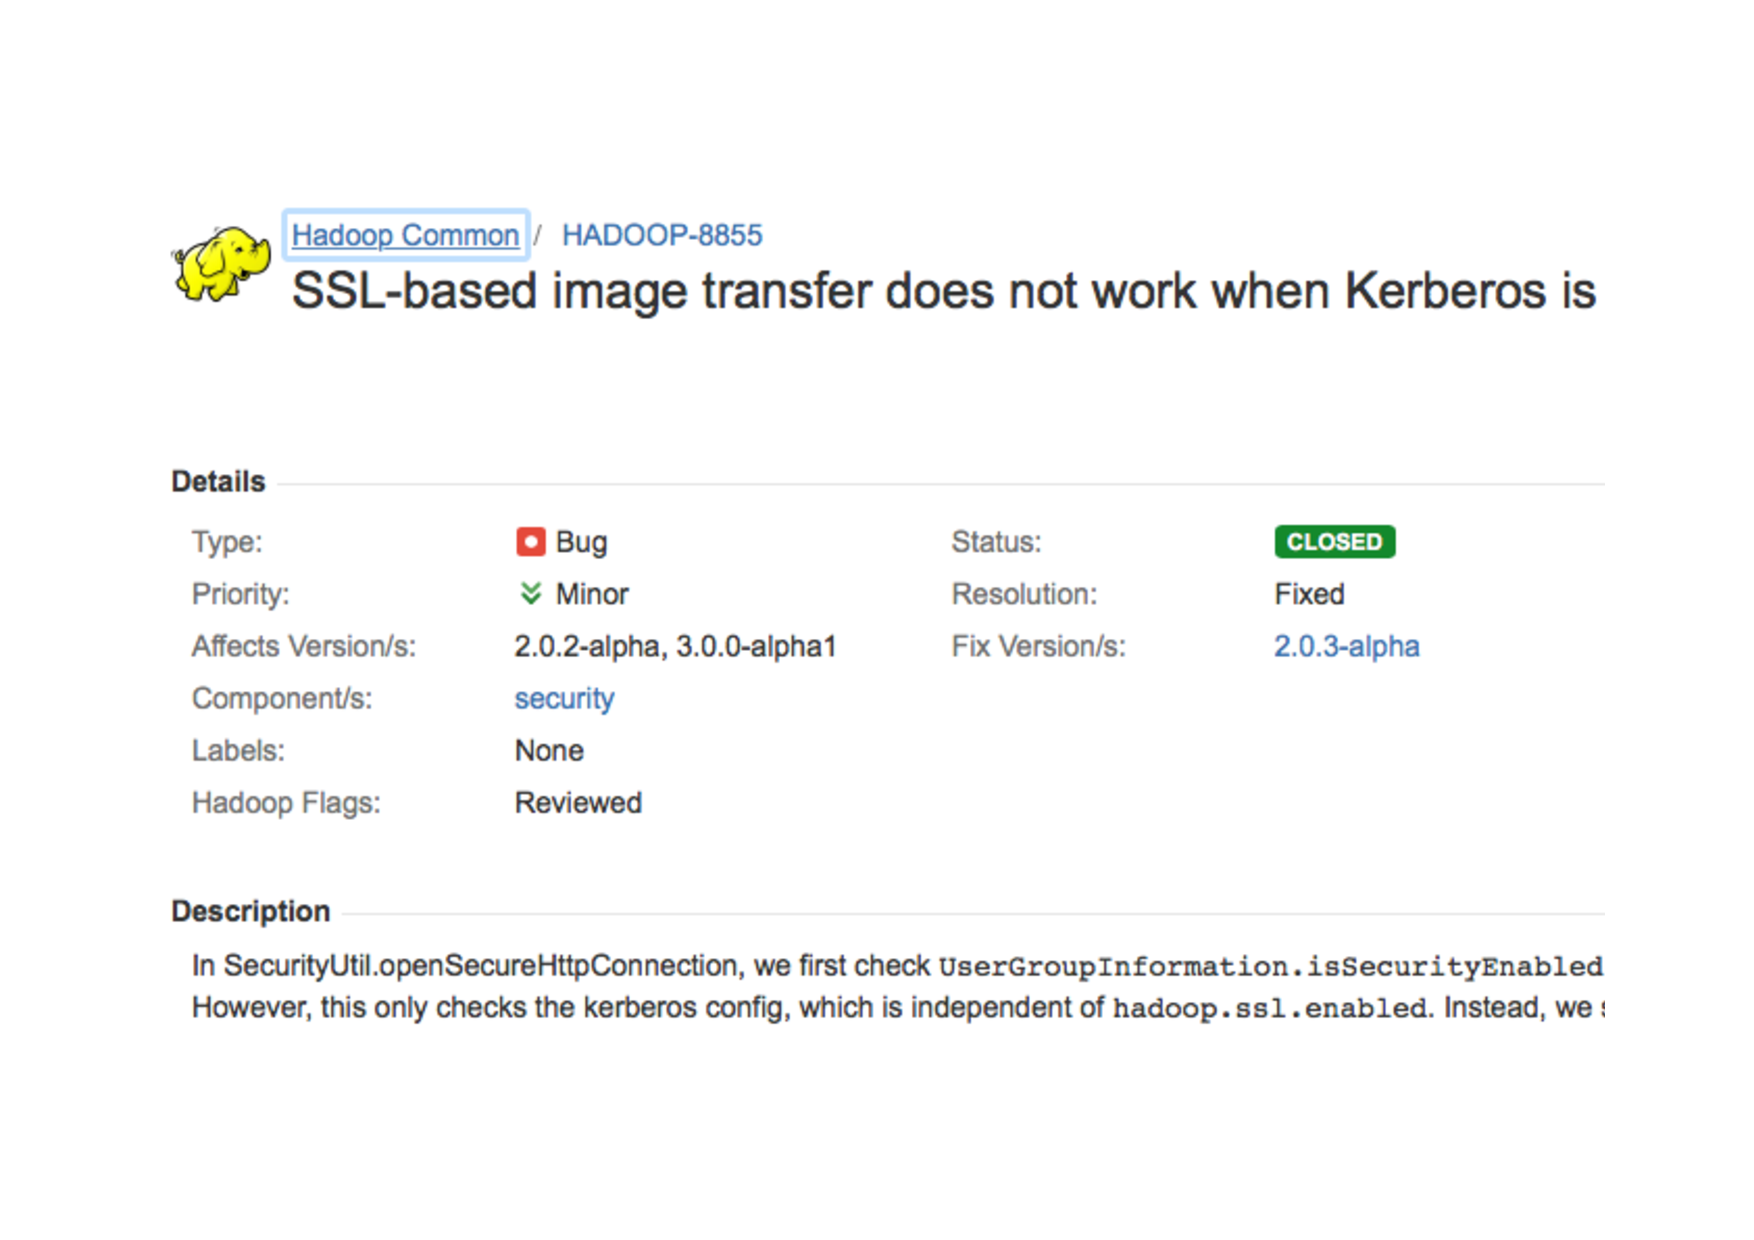
\includegraphics[width=1\textwidth]{figures/bug-report-example.pdf}
  \caption{A typical bug report (\url{https://issues.apache.org/jira/browse/HADOOP-8855}, as of September 2018)} 
  \label{fig:bug-report-example}
\end{figure}

\begin{figure}[!htp]
  \begin{subfigure}{.49\textwidth}
    \centering
    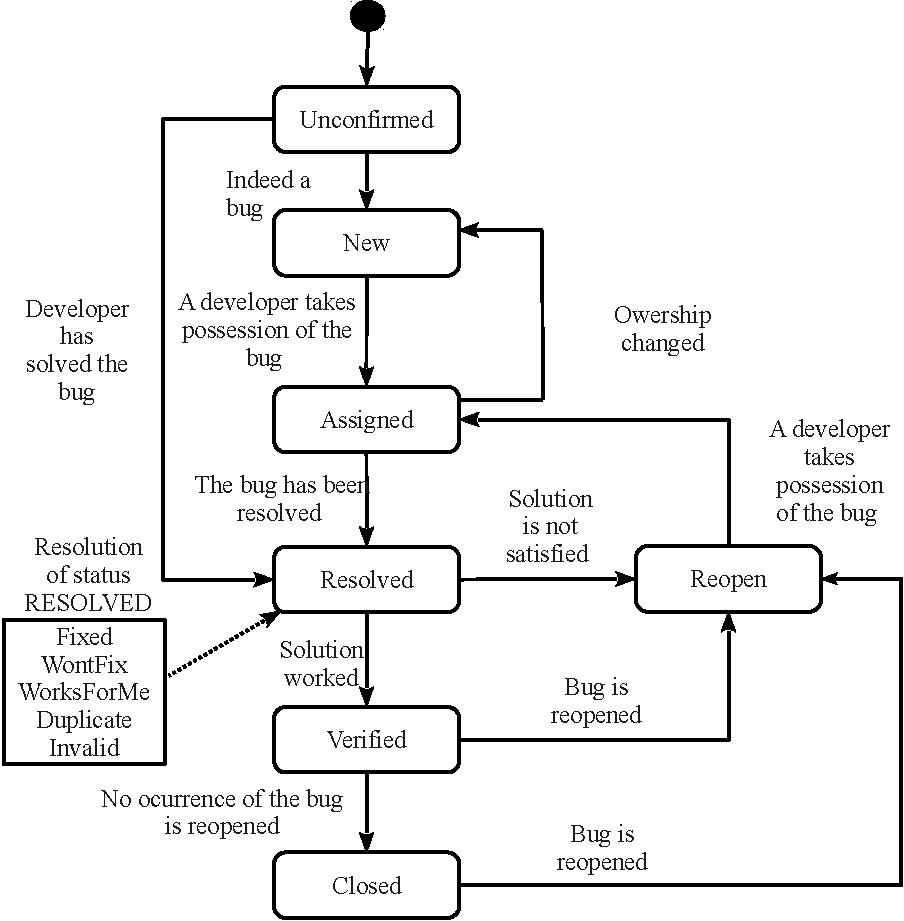
\includegraphics[width=\textwidth]{figures/bug-report-life-cycle.pdf}
    \caption{}
    \label{fig:life-cycle-of-bug-report}
  \end{subfigure}\hfill
  \begin{subfigure}{.40\textwidth}
    \centering
    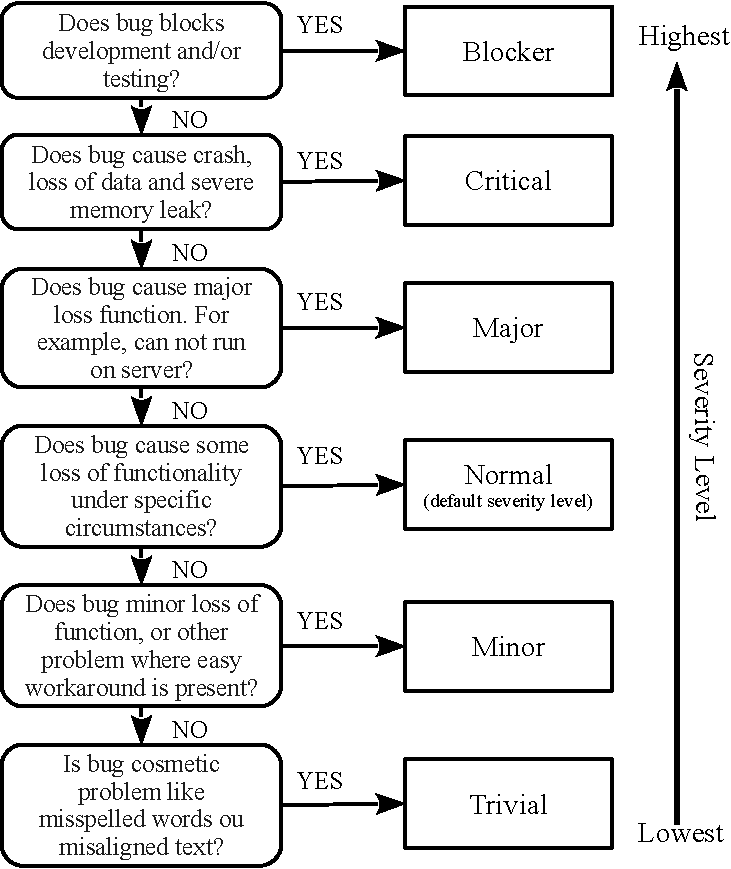
\includegraphics[width=\textwidth]{figures/bug-report-severity-levels.pdf}
    \caption{} 
    \label{fig:bug-report-severity-level-guideline}
  \end{subfigure}
  \caption{(a) The bug report lifecycle according to Zhang et al.\cite{Zhang:2015}. (b) Bugzilla guideline for bug report severity level assignment (\url{https://www.bugzilla.org}, as of \today).}
  \label{fig:bug-report-life-cycle-and-severity-level-guideline}
\end{figure}

Both users and development team members can define or redefine the severity level for a bug during the lifecycle. Figure \ref{fig:bug-report-severity-level-guideline} illustrates Bugzilla guidelines for assigning bug severity level. The Figure shows that such choices should be based on an affirmative answer to a question which characterizes a severity level appropriately. Also, the Figure indicates that \textit{Trivial} and \textit{Blocker} are lower and higher respectively.

To predict severity level, researchers sometimes aggregate these levels in severe (blocker, critical, and major) and non-severe (normal, minor and trivial) to work with a coarse-grained classification problem. Furthermore, some of them ignore the default severity level (often ``normal") because they consider this level as a choice made by users when they are not sure about the correct severity level. Other studies choose to predict a bug report severity level as \textit{blocking} or \textit{non-blocking} bug. A blocking bug is one that prevents other bugs to be fixed\cite{Valdivia:2014}. 

\subsection{Machine Learning}
Machine Learning (ML)\cite{Flach:2012} is an application of Artificial Intelligence (AI) that provides systems the ability to learn and improve from experience without being explicitly programmed. There are two types of ML algorithms: predictive (or supervised) and descriptive (or unsupervised). A predictive algorithm builds a model based on historical training data and uses this model to predict, from the values of input attributes, an output label (class attribute) for a new sample. A predictive task is called classification when the label value is discrete, or regression when the label value is continuous. 

On the other hand, a descriptive algorithm explores or describes a dataset. There is not an output label associated with a sample. Data clustering and pattern discovery are two examples of descriptive tasks. Bug report severity prediction is considered a classification problem; therefore, more detailing of descriptive algorithms are outside the scope of this paper.

\subsubsection{ML algorithms}
A ML algorithm works over a dataset, which contains many samples or instances $x_{i}$, where $i = \{1..n\}$. Each instance is composed of $\{x_{i1}, x_{i2},...,x_{id}\}$ input attributes or independent variables, where $d = \{1..m\}$, and one output attribute or dependent variable, $x_{i(m+1)}$.  Input attributes are commonly named features or feature vector, and output attribute as commonly named class or category. The most traditional ML classification algorithms are k-Nearest Neighbors, Näive Bayes, Decision Tree, Neural Networks, Random Forest and Support Vector Machine. In practice, they can be applied for both classification and regression tasks. However, this mapping review regards them only in the classification scenario. Next, a brief description of each one is presented\cite{Marsland:2014}:

\begin{itemize}
  \item \textbf{k-Nearest Neighbors} (k-NN) process the available instances (or neighbors) in a dataset and classifies a new instance based on its similarity measure to the k-nearest neighbors. Usually, k-NN algorithms utilize a Euclidean distance to quantify the proximity of neighbors. To calculate this distance, each feature vector of each instance in a dataset should represent a point of an n-dimensional space.
  
  \item \textbf{Näive Bayes} (NB) decides to which class an instance belongs based on the Bayesian Theorem of conditional probability. The probabilities of an instance belonging to each of the $C_{k}$ classes given the instance $x$ is $P(C_{k}|x )$. Näive Bayes classifiers assume that given the class variable, the value of a particular feature is independent of the value of any other feature.
  
  \item \textbf{Decision Tree} consists of a collection of internal nodes and leaf nodes in a tree, organized in a hierarchical model.  Each internal node represents a feature, and each leaf node corresponds to a class label. The decision tree classifiers organize a series of test questions and conditions in a tree structure.  A decision tree represents the model capable of guiding the decision making on the determination of the class to which an individual belongs.
  
  \item \textbf{Neural Network} is a learning algorithm that is inspired by the structure and functional aspects of biological neural networks\cite{Haykin:1998}. It structured as a network of units called neurons, with weighted, directed connections. Neural network models have been demonstrated to be capable of achieving remarkable performance in document classification\cite{Zhou:2012}.  \rem{Figure \ref{fig:artificial-neuron} presents an artificial neuron model that contains a set of weighted inputs ($w_i$), which corresponds to the synapses; an adder function ($\sum$) that sums the inputs signals; and an activation function ($f(.)$) that decides whether the neuron fires for the current inputs to generate the output value ($y_{o})$. Independent features of each instance represent neuron dendrites.}
  \rem{
  \begin{figure}[h!]
    \centering
    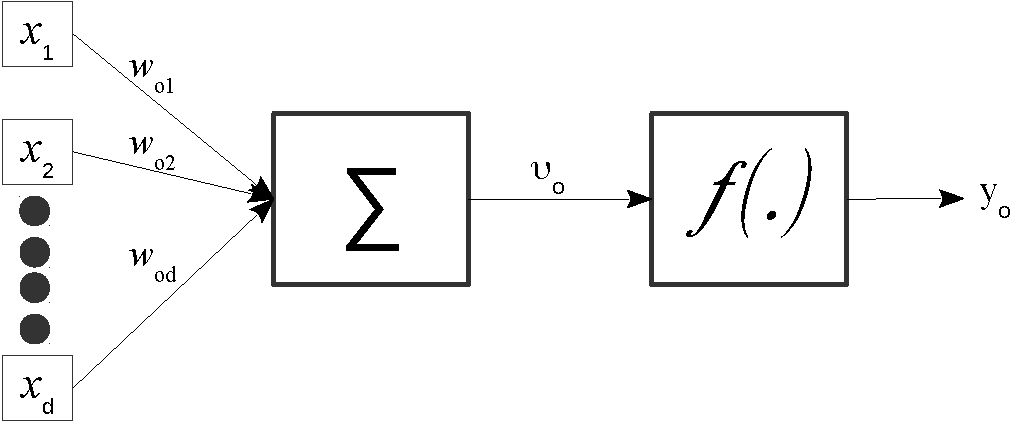
\includegraphics[width=0.5\textwidth]{figures/artificial-neuron.pdf}
    \caption{A artificial neuron model based on Marsland \cite{Marsland:2014}.}
    \label{fig:artificial-neuron}
  \end{figure}
  }
  \item \textbf{Support Vector Machine(SVM)}\rem{represents each feature vector of each instance as a point in an n-dimensional space. The algorithm divides every point belonging to a category in a particular space. Each space is separated by a gap that is as wide as possible\cite{Marsland:2014}. \rem{This space between these two regions delimits the margin between classes.}In Figure \ref{fig:support-vector-machine}, for example, SVM will search for support vectors which are instances located at the edge of an area in space. Such vectors define boundaries between one of these class instances (e.g., the crosses) and instances from another class (e.g., the circles).  \rem{Each region contains instances belonging to the same class\cite{Williams:2011}}. New instances are then mapped into that same space and predicted to belong to a category based on which side they are.}\edit{Each  feature vector of each instance is a point in an n-dimensional space.  SVM learns in this space an optimal way to separate the training instances according to their class labels. The output of this algorithm is a hyperplane, which maximizes the separation among feature vectors of instances of different classes. Given a new instance, SVM assigns a label based on which subspace  its feature vector belongs to~\cite{Tian:2016}.}
\rem{
  \begin{figure}[h!]
    \centering
    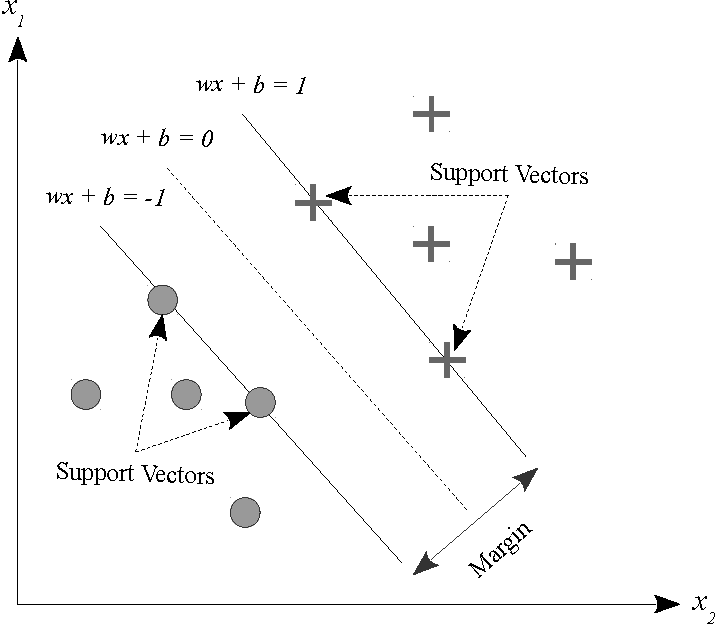
\includegraphics[width=0.4\textwidth]{figures/support-vector-machine.pdf}
    \caption{A SVM model example.}
    \label{fig:support-vector-machine}
  \end{figure}
}
  \item \textbf{Random Forest}\cite{Breiman:2001} relies on two core principles: (i) the creation of hundreds of decision trees and their combination into a single model; and (ii) the final decision is based on the ruling of the majority of the forming trees. 
\end{itemize}

\subsubsection{Feature Selection Methods}
Feature selection is the process of choosing a subset of features that better contribute to the accuracy of a predictive model. Three typical feature selection methods are described next\cite{Zheng:2004}:

\begin{itemize}
  \item \textbf{Information Gain (IG)}:  this method measures the number of bits of information obtained for category prediction by knowing the presence or absence of a feature in a dataset.
  \item \textbf{Chi-square (CHI)}: this method measures the lack of independence between a feature $f$ and category $c_i$ and can be compared to the chi-square distribution with one degree of freedom.
  \item \textbf{Correlation Coefficient (CC)}:  this method defines the correlation coefficient of feature $f$ with a category $c_i$.    
\end{itemize}

\subsubsection{Evaluation measures}
Accuracy, precision, recall, and F-measure are four measures commonly used to evaluate the performance of prediction models\cite{Feldman:2006}. The computation of the values of these measures are based on a \textit{confusion matrix}\cite{Williams:2011}, which represents the number of true/false positives, and the number of true/false negatives for each instance class value when making a prediction. Each measure is described next \cite{Japkowicz:2011}: 

\begin{itemize}
  \item \textbf{Accuracy} is the percentage of correctly classified observations among all observations:
  
  \begin{equation}
  Accuracy = \frac{TP+TN}{P+N}
  \end{equation}
  
  where P is the total of positive class instances, N is the total of negative class instances, TP is the number of true positives, and TN is the number of true negatives.
  
  \item \textbf{Precision} is the percentage of correctly classified observations among all observations that were assigned to the class by the classifier. It can be viewed as a measure of classifier exactness. A low precision can also indicate a large number of false positives. More formally recall is defined as:
  
  \begin{equation}
  Precision = \frac{TP}{TP+FP}
  \end{equation}
  
  where TP is the number of true positives, and FP is the number of false positives.
  
  \item \textbf{Recall} of a classification method can be defined as the percentage of correctly classified observations among all observations belonging to that class. It can be viewed as a measure of a classifiers completeness. A low recall indicates many false negatives in testing classification step. More formally recall is defined as: 
  
  \begin{equation}
  Recall = \frac{TP}{TP+FN}
  \end{equation}
  
  where TP is the number of true positives, and FN is the number of false negatives.
  
  \item \textbf{F-measure} is a harmonic mean of the precision and recall\cite{Feldman:2006}. F-measure can be calculated as:
  
  \begin{equation}
  \textit{F-measure} = \frac{2 \times (precision \times recall)}{(precision + recall)}
  \end{equation}
  
\end{itemize}

Receiving Operating Characteristics (ROC) is an alternative measure to evaluate binary classifiers. A ROC curve\cite{Japkowicz:2011} is a bidimensional chart, where the X-axis represents false positives, and the Y-axis represents true positives. The Area Under ROC Curve (AUC), ranging between 0 and 1, is used to assess the performance of ML algorithms. An algorithm outperforms another one if its AUC value is closer to 1. 

\subsubsection{Sampling methods}
The evaluation of the supervised method effectiveness is mainly based on two datasets with labeled samples, one for training the predictive model and the other for testing this model. Assessing performance of a predictive model using the same dataset for training and testing is not recommend and may yield misleading optimistic estimations\cite{Japkowicz:2011}. In order to obtain more reliable predictive estimates, resampling methods can be used to split the entire dataset into a training dataset and a testing dataset. Such methods according to  Facelli et al. \cite{Facelli:2015} include: 
\begin{itemize} 
  \item \textbf{Holdout} splits a dataset into a ratio of \textit{p} for training and $(1 - p)$ for testing. 
  \item \textbf{Cross-Validation (CV)} divides a dataset into $k$ folds. In each iteration, it saves a different fold for testing and uses all the others for training. 
  \item \textbf{Bootstrap} generates \textit{r} training subsets from the original dataset. It randomly samples instances with replacement from this set. Unselected cases make up the test subset. The result is the average performance observed for each test subset.
\end{itemize}

\subsubsection{Statistical tests}
\edit{Many scenarios require running several ML algorithms to chose the best predictive model. Even though the performance of these algorithms may be shown to be different on specific datasets, it needs to be confirmed whether the observed differences are statistically significant and not merely coincidental\cite{Japkowicz:2011}. In this situation, conducting statistical tests is a recommended practice for reliable comparison between predictive models under investigation\cite{Facelli:2015}. A brief description of four common statistical tests is provided:}

\begin{itemize}
  \item \textbf{T-Test}\cite{Japkowicz:2011} is a parametric statistical hypothesis test that can be used to assess whether the means of two groups are statistically different from each other.
  \item \textbf{Wilcoxon signed-rank test}\cite{Wilcoxon:1992} is a non-parametric statistical hypothesis test that can be used to determine whether two dependent samples, selected from the population, have the same distribution. 
  \item \textbf{Proportion test}\cite{Lewis:2013} is a parametric statistical hypothesis test that can be used to assess whether or not a sample from a population represents the true proportion of the entire population. 
  \item \textbf{Shapiro Wilk test}\cite{Lewis:2013} is a parametric statistical hypothesis test that can be used to test whether a sample $x_1, ..., x_n$ came from a normal distribution of the population.
\end{itemize}


\subsection{Text Mining}
The common ML algorithms cannot directly process unstructured text (e.g., \textit{summary} and \textit{description} fields from bug report form). Therefore, during a preprocessing step, these unstructured text fields are converted into more manageable representations. Typically, the content of these fields is represented by feature vectors, points of an n-dimensional space. Text mining is the process of converting unstructured text into a structure suited to analysis\cite{Feldman:2006}. It is composed of three primary activities\cite{Williams:2011}:

\begin{itemize}
  \item \textbf{Tokenization} is the action to parsing a character stream into a sequence of tokens by splitting the stream at delimiters. A token is a block of text or a string of characters (without delimiters such as spaces and punctuation), which is a useful portion of the unstructured data. 
  \item \textbf{Stop words removal} eliminates commonly used words that do not provide relevant information to a particular context, including prepositions, conjunctions, articles, common verbs, nouns, pronouns, adverbs, and adjectives. 
  \item \textbf{Stemming} is the process of reducing or normalizing inflected (or sometimes derived) words to their word stem, base form—generally a written word form (e.g., ``working” and ``worked" into ``work").
\end{itemize}

Two of the most traditional ways of representing a document relies on the use of a bag of words (unigrams) or a bag of bigrams (when two terms appear consecutively, one after the other)\cite{Feldman:2006}. In this approach all terms represent features, and thus the dimension of the feature space is equal to the number of different terms in all documents (bug reports). Methods for assigning weights to features may vary. The simplest one is to assign binary values representing the presence or absence of the term in each text. Term Frequency (TF), another type of quantification scheme, considers the number of times in which the term appears in each document. Term Frequency-Inverse Document Frequency (TD-IDF), a more complex type of scheme,  takes into account the frequencies of the term in each document, and in the whole collection.  The importance of a term in this scheme is proportional to its frequency in the document and inversely proportional to the frequency of the term in the collection. 
\section{Experiment} \label{sec:experiment}
This section describes the experiment conducted to address the Research Questions. As in typical methodologies used in ML studies, it comprises the following steps: Data Collection (\ref{subsec:collection}), Data Preprocessing (Section \ref{subsec:preprocessing}), and Training and Testing (Section \ref{subsec:training}).

\subsection{Data Collection} 	\label{subsec:collection}
This step in the experimental research encompasses selecting FLOSS datasets to serve as the data source, studying and interpreting its data structure, and finally extracting relevant data from its repository (feature extraction). In this research, Cassandra, Hadoop, Linux, Mozilla, and Spark Open Systems were considered as potential Open Source Systems to study. In a first approximation, Cassandra, Hadoop and Spark were selected as data sources of CR records, due to the fact they are open, well stablished, have a considerable number of CRs already registered, use standard repositories, and were under study by other researchers in our research group.

Cassandra[cassandra.apache.org] is a distributed NoSQL database management system designed to handle large amounts of data across many servers, providing fault-tolerance with no single point of failure. Hadoop[hadoop.apache.org] is a framework that allows for the distributed processing of large data sets across clusters of computers using simple programming models. Spark[spark.apache.org] is a cluster-computing engine for large-scale data processing which provides an interface for programming entire clusters with implicit data parallelism and fault-tolerance. They are considered a specialized and complex FLOSS project with many users with different levels of expertise.

CRs from these FLOSS projects are stored in a Jira based repository [\url{https://www.atlassian.com/software/jira}] which allows for access to all CR contents in XML format. Everything is available (except change history), from CR long description field (with lines with few characters to ones with many lines), including code snippets and exception stack trace. Two steps are used to perform data extraction from their web site[\url{http://issues.apache.org}]: (i) copying CR basic data (e.g. status and resolution) from XML contents; and (ii) copying CR changes history from external HTML pages (this may be important for learning).

CR record data from February 01, 2006 to May 07, 2017 were collected.  The total number of CR records retrieved after preprocessing was 22901. 
 
\begin{figure*}[!ht]
  \centering
  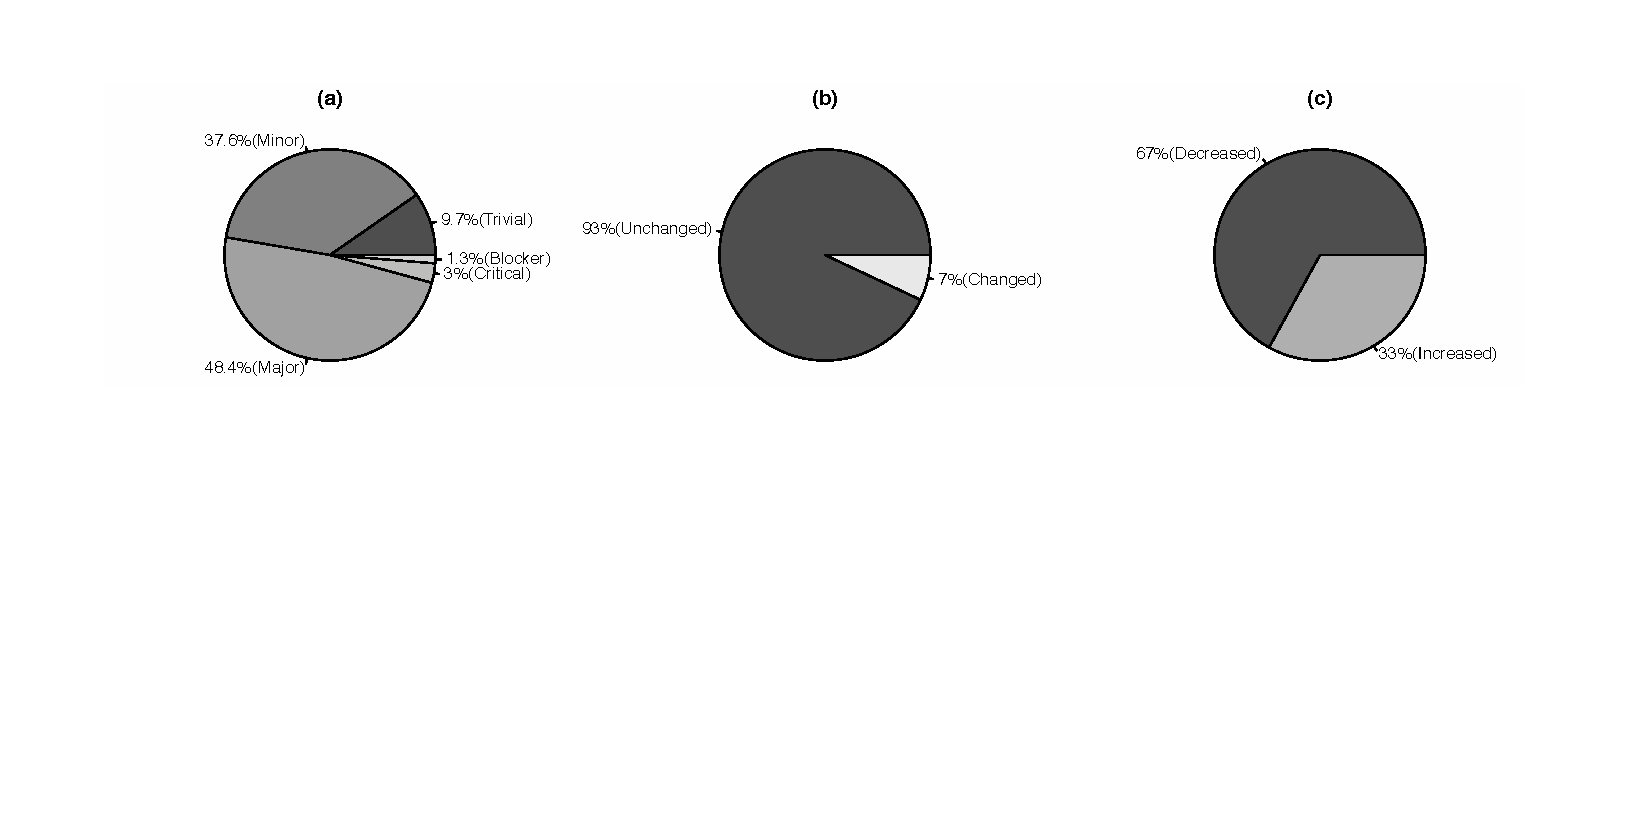
\includegraphics[scale=0.7]{figures/issues_distribution_cassandra.pdf}    
  \caption{Cassandra dataset distributions: (a) severity level (b) change pattern (c) direction of change.}
  \label{fig:issues_distribution_cassandra}
\end{figure*}

\begin{figure*}[!ht]
  \centering
  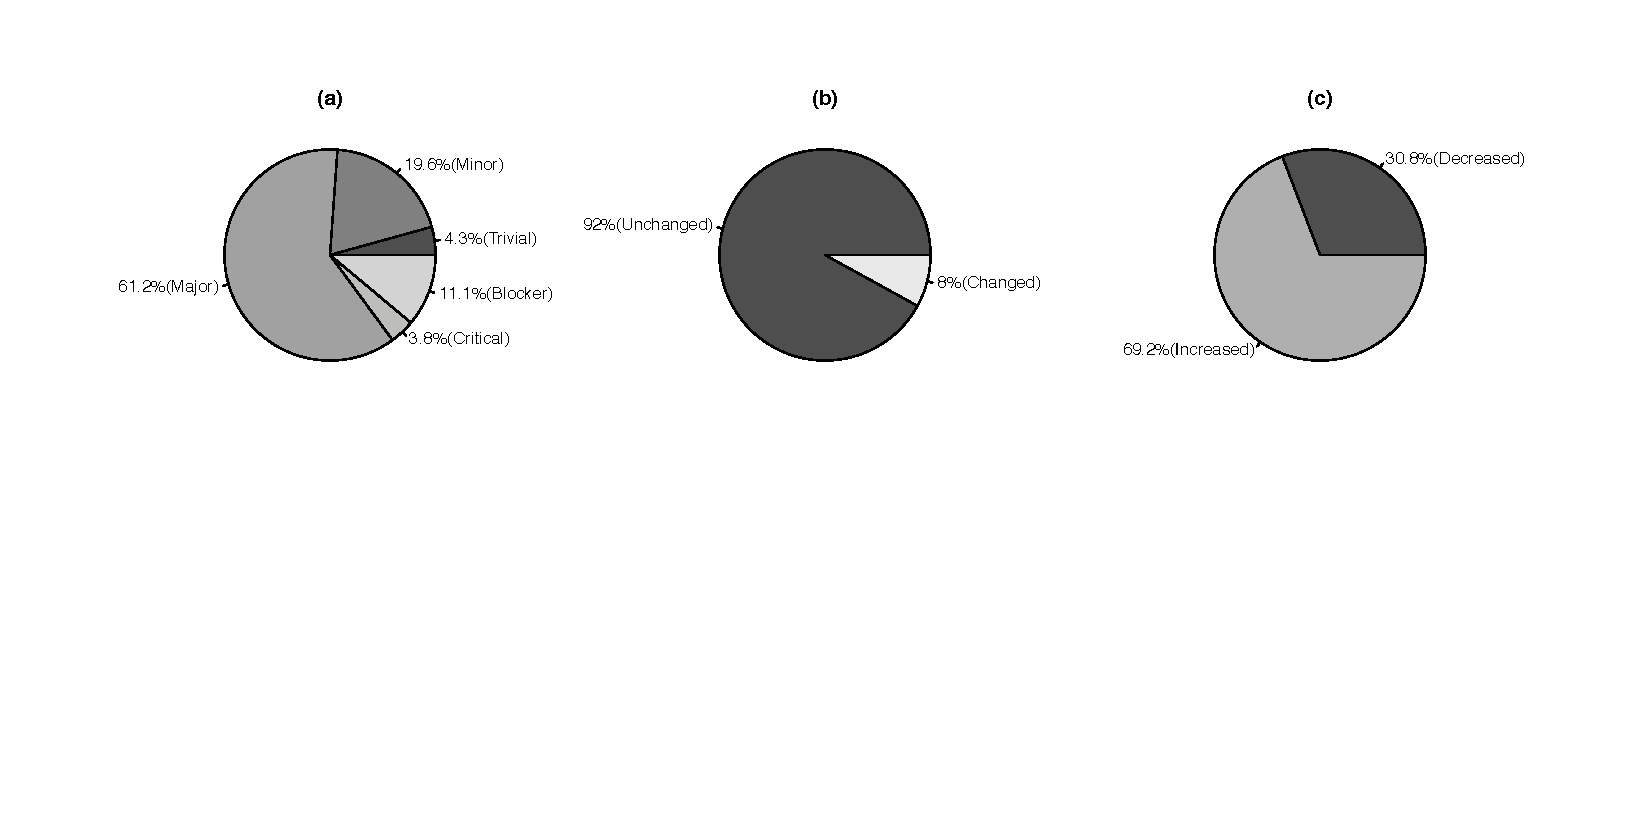
\includegraphics[scale=0.7]{figures/issues_distribution_hadoop.pdf}
  \caption{Hadoop dataset distributions: (a) severity level (b) change pattern (c) direction of change.}
  \label{fig:issues_distribution_hadoop}
\end{figure*}

\begin{figure*}[!ht]
  \centering
  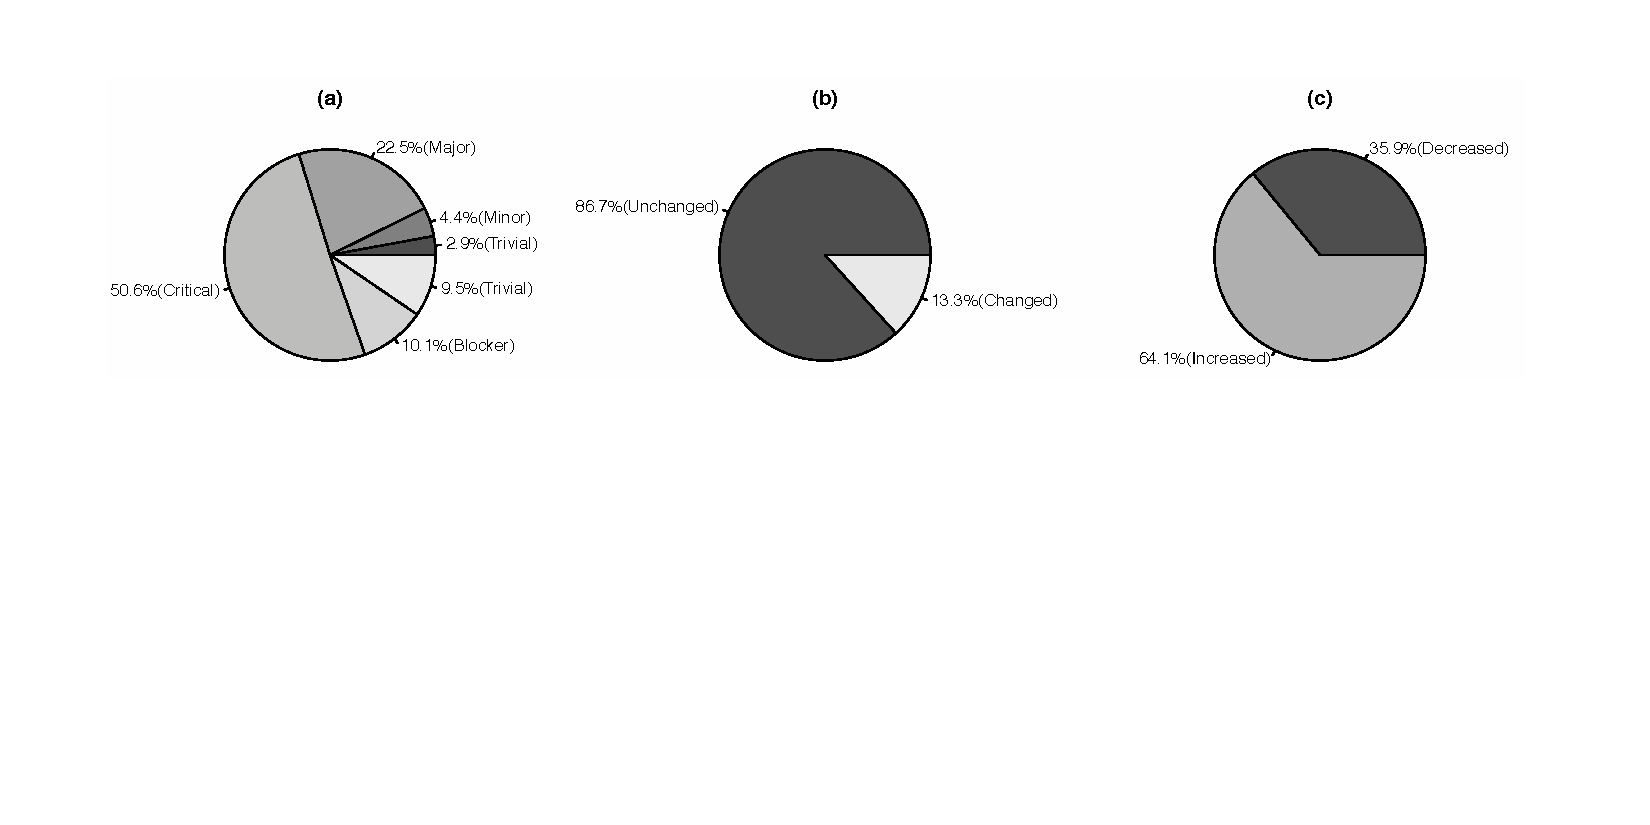
\includegraphics[scale=0.7]{figures/issues_distribution_spark.pdf}   
  \caption{Spark dataset distributions: (a) severity level (b) change pattern (c) direction of change.}
  \label{fig:issues_distribution_spark}
\end{figure*}


Figure \ref{fig:issues_distribution_cassandra} shows how the 7538 retrieved CR Cassandra records were distributed in terms of severity level and severity level change. Figure \ref{fig:issues_distribution_cassandra}(a) shows the severity level distribution: 9.7\% have severity trivial (1); 37.6\% have severity minor (2); 48.4\% have severity major (3), 3.0\% have severity critical (4), and 1.3\% have severity blocker (5). Figure \ref{fig:issues_distribution_cassandra}(b) shows that only 7.0\% have changed their severities levels during the CR lifecycle. Finally, Figure \ref{fig:issues_distribution_cassandra}(c) reveals that of these 7.0\% CRs which changed their severity, 67\% decreased it, and 33\% increased it. 

Figure \ref{fig:issues_distribution_hadoop} shows how the 8262 retrieved CR Hadoop records from were distributed in terms of severity level and severity level change. Figure \ref{fig:issues_distribution_hadoop}(a) shows the severity level distribution: 4.3\% have severity trivial (1); 19.6\% have severity minor (2); 61.2\% have severity major (3), 3.8\% have severity critical (4), and 11.1\% have severity blocker (5). Figure \ref{fig:issues_distribution_hadoop}(b) shows that only 8.0\% have changed their severities levels during the CR lifecycle. Finally, Figure \ref{fig:issues_distribution_hadoop}(c) reveals that of these 8.0\% CRs which changed their severity, 30.8\% decreased it, and 69.2\% increased it. 

Figure \ref{fig:issues_distribution_spark} shows how the 7101 retrieved CR Spark records were distributed in terms of severity level and severity level change. Figure \ref{fig:issues_distribution_spark}(a) shows the severity level distribution: 2.9\% have severity trivial (1); 4.4\% have severity minor (2); 22.5\% have severity major (3), 50.6\% have severity critical (4), and 10.1\% have severity blocker (5). Figure \ref{fig:issues_distribution_spark}(b) shows that only 13.3\% have changed their severities levels during the CR lifecycle. Finally, Figure \ref{fig:issues_distribution_spark}(c) reveals that of these 13.3\% CRs which changed their severity, 35.9\% decreased it, and 64.1\% increased it. 

Summarizing findings in Figures \ref{fig:issues_distribution_cassandra}, \ref{fig:issues_distribution_hadoop} and  \ref{fig:issues_distribution_spark}: (a) the most frequent severity level type is ``major''; (b) there have been few changes in severity levels; (c) in two of them (Hadoop and Spark), severity levels increased. Furthermore, one can see that these datasets are clearly imbalanced, posing additional difficulty to the application of the ML methodology. 

\subsection{Preprocessing} 	\label{subsec:preprocessing}

Raw data previously collected from the Cassandra, Hadoop and Spark CR repositories were not properly structured to serve as input to ML algorithms, they weren't in tidy data format \cite{DeJonge2013}. The classical way to address this problem is to run preprocessing procedures to extract, organize and structure relevant features out of the raw data. Specific scripts were written in R language to accomplish this features extraction. Preprocessing tasks were executed as follows:  

\begin{itemize}
 \item Extraction of relevant features: key, type, status, resolution status, days to resolve, quantity of comments, severity level and long description of CRs; 
 \item Selecting only CRs with status equals to Closed and resolution equals to Fixed and Implemented. This type of CRs was effectively implemented by the development team and they can no longer have their severity level changed.
 \item Merging CR features with their change history data. This additional information allows for the identification of CRs that have changed severity level during the CR lifecycle, and furthermore, if they have changed for better (decrease) or worse (increase).
 \item Performing text mining in the long description field to identify the 100 most frequent words. This information is then converted into features for each CR.
\end{itemize}

\subsection{Training and testing}  	\label{subsec:training}

Training and testing steps start with partitioning the already preprocessed dataset in two disjoint subsets: a subset for training, with 80\% of the CRs, and a subset for testing, with the remaining 20\% of the CRs. Three classical sampling approaches, random, proportional, and uniform\cite{Japkowicz:2011} were analyzed to select the training set. Best results were obtained with the random sampling technique. In the training phase, we have used the 5$\times$3 Repeated Cross-Validation technique \cite{Zhao2013} to obtain more stable estimates of each algorithm's performance and enhance replicability of the results \cite{Japkowicz:2011}. In the testing phase, each ML algorithm was validated with 20\% of each CR dataset to measure its accuracy.
 
We have chosen three traditional ML algorithms: Neural Networks\cite{Haykin:1998}, Random Forest\cite{Breiman2001} and Support Vector Machine(SVM)\cite{Cristianini:1999} which were implemented, respectively, using neuralnet (with Single Hidden Layer), randomForest, and kernlab (with Radial Basis Function Kernel and multi-class classification) R libraries.




\section{Findings and Discussions}  \label{sec:discussion}
This section presents the experimental findings listed by research question: RQ1 (\ref{subsec:rq1}), RQ2 (Section \ref{subsec:rq2}), RQ3 (Section \ref{subsec:rq3}) and RQ4 (Section \ref{subsec:rq4}). In addition, the performance of ML algorithms is evaluated using Friedman Statistical Test (Section \ref{subsec:tests}). 

\subsection{RQ1: Will the CR severity level change?}\label{subsec:rq1}

The RQ1 is a simple binary problem, i.e., a question whose answer is true (class 1) or false (class 0). Tables \ref{tab:classifiers_precision_on_rq1}, \ref{tab:classifiers_recall_on_rq1} and \ref{tab:classifiers_f_measure_on_rq1} 
show the performance of ML algorithms to predict the response to this issue.

\begin{table}[!ht]
	\renewcommand{\arraystretch}{1.8}
	\caption{ML algorithms precision performance on RQ1.}
	\label{tab:classifiers_precision_on_rq1}
	\centering
	\begin{tabular}{l|c|c|c|c|}
		\cline{2-5}
		& Class & Neural Network & Random Forest & SVM\\
		\cline{1-5}
		\multicolumn{5}{ |c| }{Precision}\\
		\cline{1-5} 
        \multicolumn{1}{ |c| }{\multirow{2}{*}{\rotatebox[origin=c]{90}{\scriptsize{Cassandra}}}} & 0 & 0.9530591 & 0.9596013 & 0.9581371\\
		\cline{2-5}
		\multicolumn{1}{ |c| }{} & 1 & 0.7241379 & 0.9740260 & 1.0000000\\
		\hline
		\multicolumn{1}{ |c| }{\multirow{2}{*}{\rotatebox[origin=c]{90}{\scriptsize{Hadoop}}}} & 0 & 0.9530516 & 0.9498208 & 0.9477157\\
		\cline{2-5}
		\multicolumn{1}{ |c| }{} & 1 & 0.6339286 & 0.8289474 & 0.9830508\\
		\hline
		\multicolumn{1}{ |c| }{\multirow{2}{*}{\rotatebox[origin=c]{90}{\scriptsize{Spark}}}} 		
		& 0 & 0.9125249 & 0.9274406 & 0.9134555\\
		\cline{2-5}
		\multicolumn{1}{ |c| }{} & 1 & 0.6162162 & 0.7640449 & 0.9819820\\
		\cline{1-5} 
		\multicolumn{1}{ |c| }{} & Average & 0.7988197 & 0.9006468 & 0.9640569\\
		\hline 
	\end{tabular}
\end{table}
%
\begin{table}[!ht]
	\renewcommand{\arraystretch}{1.8}
	\caption{ML algorithms recall performance on RQ1.}
	\label{tab:classifiers_recall_on_rq1}
	\centering
	\begin{tabular}{l|c|c|c|c|}
		\cline{2-5}
		& Class & Neural Network & Random Forest & SVM\\
		\cline{1-5}		
		\multicolumn{5}{ |c| }{Recall}\\
		\cline{1-5} 
        \multicolumn{1}{ |c| }{\multirow{2}{*}{\rotatebox[origin=c]{90}{\scriptsize{Cassandra}}}} & 0 & 0.9868924 & 0.9989077 & 1.0000000\\
		\cline{2-5}
		\multicolumn{1}{ |c| }{} & 1 & 0.4144737 & 0.4934211 & 0.4736842\\
		\hline
		\multicolumn{1}{ |c| }{\multirow{2}{*}{\rotatebox[origin=c]{90}{\scriptsize{Hadoop}}}} & 0 & 0.9780514 & 0.9930407 & 0.9994647\\
		\cline{2-5}
		\multicolumn{1}{ |c| }{} & 1 & 0.4409938 & 0.3913043 & 0.3602484\\
		\hline
		\multicolumn{1}{ |c| }{\multirow{2}{*}{\rotatebox[origin=c]{90}{\scriptsize{Spark}}}} 		
		& 0 & 0.9509669 & 0.9709945 & 0.9986188\\
		\cline{2-5}
		\multicolumn{1}{ |c| }{} & 1 & 0.4634146 & 0.5528455 & 0.4430894\\
		\cline{1-5} 
		\multicolumn{1}{ |c| }{} & Average & 0.7057988 & 0.7334190 & 0.7125176\\
		\hline 
	\end{tabular}
\end{table}
%
\begin{table}[!ht]
	\renewcommand{\arraystretch}{1.8}
	\caption{ML algorithms F-measure performance on RQ1.}
	\label{tab:classifiers_f_measure_on_rq1}
	\centering
	\begin{tabular}{l|c|c|c|c|}
		\cline{2-5}
		& Class & Neural Network & Random Forest & SVM\\
		\cline{1-5}		
		\multicolumn{5}{ |c| }{F-measure}\\
		\cline{1-5} 
        \multicolumn{1}{ |c| }{\multirow{2}{*}{\rotatebox[origin=c]{90}{\scriptsize{Cassandra}}}} & 0 & 0.9696807 & 0.9788600 & 0.9786211\\
		\cline{2-5}
		\multicolumn{1}{ |c| }{} & 1 & 0.5271967 & 0.6550218 & 0.6428571\\
		\hline
		\multicolumn{1}{ |c| }{\multirow{2}{*}{\rotatebox[origin=c]{90}{\scriptsize{Hadoop}}}} & 0 & 0.9653897 & 0.9709500 & 0.9729026\\
		\cline{2-5}
		\multicolumn{1}{ |c| }{} & 1 & 0.5201465 & 0.5316456 & 0.5272727\\
		\hline
		\multicolumn{1}{ |c| }{\multirow{2}{*}{\rotatebox[origin=c]{90}{\scriptsize{Spark}}}} 		
		& 0 & 0.9313493 & 0.9487179 & 0.9541405\\
		\cline{2-5}
		\multicolumn{1}{ |c| }{} & 1 & 0.5290023 & 0.6415094 & 0.6106443\\
		\cline{1-5} 
		\multicolumn{1}{ |c| }{} & Average & 0.7404609 & 0.7877841 & 0.7810730\\
		\hline 
	\end{tabular}
\end{table}

We tested the ML algorithms with 4580 (20\% of 22901) CRs: 4154 have changed their severity level, and 426 haven't changed their severity level. We can observe that the three algorithms performed very closely. However, the Random Forest algorithm had the best performance in two out of three measures. 

We have also analyzed the percentage of incorrect predictions made in answering RQ1. Figure \ref{fig:classifiers_performance_on_q1q2q3} shows that this implementation of the Neural Network Algorithm had the worst performance and the two others performed similarly. 

\begin{figure*}[!ht]
  \centering
  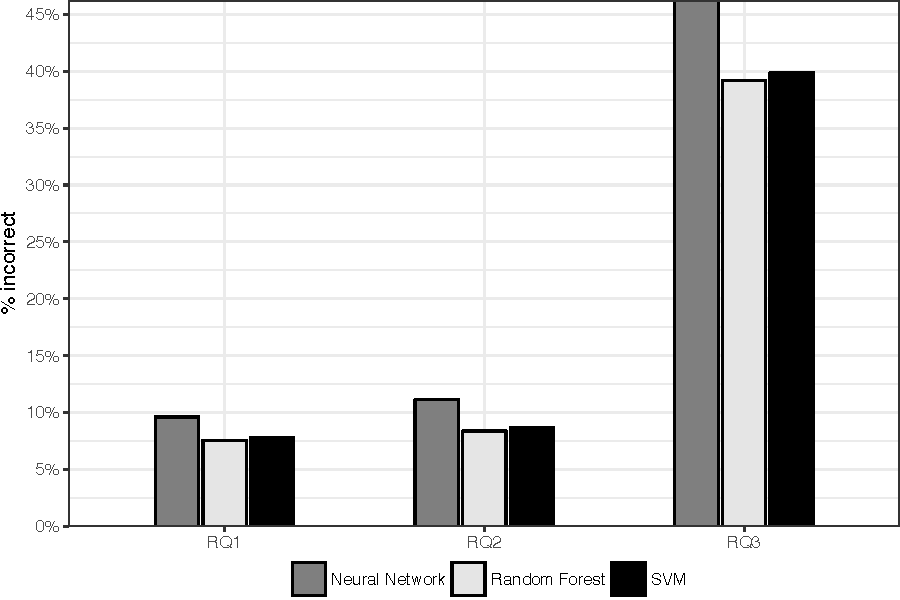
\includegraphics[scale=1]{figures/classifiers_performance_on_q1q2q3.pdf}
  \caption{Performance of ML algorithms for RQ1 and RQ2.}
  \label{fig:classifiers_performance_on_q1q2q3}
\end{figure*}

\subsection{RQ2: Will the CR severity level increase, decrease or remain the same?}\label{subsec:rq2}

The RQ2 poses a problem more difficult than the previous question. It is a question with three possible responses related to severity level: it has decreased (class -1); it has remained (class 0); and it has increased (class 1). Tables \ref{tab:classifiers_precision_on_rq2}, \ref{tab:classifiers_recall_on_rq2}, and \ref{tab:classifiers_f_measure_on_rq2} shows the performance of the ML algorithms to predict the response to this issue. 

\begin{table}[!ht]
	\renewcommand{\arraystretch}{1.8}
	\caption{ML algorithms precision performance on RQ2.}
	\label{tab:classifiers_precision_on_rq2}
	\centering
	\begin{tabular}{l|c|c|c|c|}
		\cline{2-5}
		& Class & Neural Network & Random Forest & SVM\\
		\cline{1-5}	
		\multicolumn{5}{ |c| }{Precision}\\
		\cline{1-5} 
        \multicolumn{1}{ |c| }{\multirow{3}{*}{\rotatebox[origin=c]{90}{\scriptsize{Cassandra}}}} & -1 & 0.4393939 & 0.7435897 & 0.7631579\\
		\cline{2-5}
		\multicolumn{1}{ |c| }{} & 0 & 0.9523305 & 0.9565445 & 0.9546403\\
		\cline{2-5}
		\multicolumn{1}{ |c| }{} & 1 & 0.7333333 & 0.7428571 & 0.8214286\\
		\hline
		\multicolumn{1}{ |c| }{\multirow{3}{*}{\rotatebox[origin=c]{90}{\scriptsize{Hadoop}}}} & -1 & 0.2272727 & 0.5555556 & 0.5000000\\
		\cline{2-5}
		\multicolumn{1}{ |c| }{} & 0 & 0.9549266 & 0.9551084 & 0.9520653\\
		\cline{2-5}
		\multicolumn{1}{ |c| }{} & 1 & 0.6060606 & 0.7195122 & 0.8666667\\
        \hline
		\multicolumn{1}{ |c| }{\multirow{2}{*}{\rotatebox[origin=c]{90}{\scriptsize{Spark}}}} 	& -1 & 0.2500000 & 0.5925926 & 0.5769231\\
		\cline{2-5}
		\multicolumn{1}{ |c| }{} & 0 & 0.9119788 & 0.9303548 & 0.9157695\\
		\cline{2-5}
		\multicolumn{1}{ |c| }{} & 1 & 0.5555556 & 0.6689655 & 0.7977528\\
		\cline{1-5} 
		\multicolumn{1}{ |c| }{} & Average & 0.6256502 & 0.7627867 & 0.7942671\\
		\hline
	\end{tabular}
\end{table}

\begin{table}[!ht]
	\renewcommand{\arraystretch}{1.8}
	\caption{ML algorithms recall performance on RQ2.}
	\label{tab:classifiers_recall_on_rq2}
	\centering
	\begin{tabular}{l|c|c|c|c|}
		\cline{2-5}
		& Class & Neural Network & Random Forest & SVM\\
		\cline{1-5}	
		\multicolumn{5}{ |c| }{Recall}\\
		\cline{1-5} 
        \multicolumn{1}{ |c| }{\multirow{3}{*}{\rotatebox[origin=c]{90}{\scriptsize{Cassandra}}}} & -1 & 0.2989691 & 0.2989691 & 0.29896907\\
		\cline{2-5}
		\multicolumn{1}{ |c| }{} & 0 & 0.9819771 & 0.9978154 & 1.00000000\\
		\cline{2-5}
		\multicolumn{1}{ |c| }{} & 1 & 0.3928571 & 0.4642857 & 0.41071429\\
		\hline
		\multicolumn{1}{ |c| }{\multirow{3}{*}{\rotatebox[origin=c]{90}{\scriptsize{Hadoop}}}} & -1 & 0.1111111 & 0.1111111 & 0.08888889\\
		\cline{2-5}
		\multicolumn{1}{ |c| }{} & 0 & 0.9753747 & 0.9908994 & 0.99946467\\
		\cline{2-5}
		\multicolumn{1}{ |c| }{} & 1 & 0.5172414 & 0.5086207 & 0.44827586\\
        \hline
		\multicolumn{1}{ |c| }{\multirow{2}{*}{\rotatebox[origin=c]{90}{\scriptsize{Spark}}}} 	& -1 & 0.1500000 & 0.2000000 & 0.18750000\\
		\cline{2-5}
		\multicolumn{1}{ |c| }{} & 0 & 0.9516575 & 0.9779006 & 0.99861878\\
		\cline{2-5}
		\multicolumn{1}{ |c| }{} & 1 & 0.4518072 & 0.5843373 & 0.42771084\\
		\cline{1-5} 
		\multicolumn{1}{ |c| }{} & Average & 0.5367772 & 0.5704376 & 0.5400158\\
		\hline
	\end{tabular}
\end{table}

\begin{table}[!ht]
	\renewcommand{\arraystretch}{1.8}
	\caption{ML algorithms F-measure performance on RQ2.}
	\label{tab:classifiers_f_measure_on_rq2}
	\centering
	\begin{tabular}{l|c|c|c|c|}
		\cline{2-5}
		& Class & Neural Network & Random Forest & SVM\\
		\cline{1-5}	
		\multicolumn{5}{ |c| }{F-measure}\\
		\cline{1-5} 
        \multicolumn{1}{ |c| }{\multirow{3}{*}{\rotatebox[origin=c]{90}{\scriptsize{Cassandra}}}} & -1 & 0.3558282 & 0.4264706 & 0.4296296\\
		\cline{2-5}
		\multicolumn{1}{ |c| }{} & 0 & 0.9669266 & 0.9767442 & 0.9767938\\
		\cline{2-5}
		\multicolumn{1}{ |c| }{} & 1 & 0.5116279 & 0.5714286 & 0.5476190\\
		\hline
		\multicolumn{1}{ |c| }{\multirow{3}{*}{\rotatebox[origin=c]{90}{\scriptsize{Hadoop}}}} & -1 & 0.1492537 & 0.1851852 & 0.1509434\\
		\cline{2-5}
		\multicolumn{1}{ |c| }{} & 0 & 0.9650424 & 0.9726747 & 0.9751893\\
		\cline{2-5}
		\multicolumn{1}{ |c| }{} & 1 & 0.5581395 & 0.5959596 & 0.5909091\\
        \hline
		\multicolumn{1}{ |c| }{\multirow{2}{*}{\rotatebox[origin=c]{90}{\scriptsize{Spark}}}} 	& -1 & 0.1875000 & 0.2990654 & 0.2830189\\
		\cline{2-5}
		\multicolumn{1}{ |c| }{} & 0 & 0.9313957 & 0.9535354 & 0.5290023\\
		\cline{2-5}
		\multicolumn{1}{ |c| }{} & 1 & 0.4983389 & 0.6237942 & 0.5568627\\
		\cline{1-5} 
		\multicolumn{1}{ |c| }{} & Average & 0.5693392 & 0.6227619 & 0.6073741\\
		\hline
	\end{tabular}
\end{table}

We tested the ML algorithms with 4580 (20\% of 22901) CR. Only now, we have three predicting situations: 4154 haven't changed their severity level, 246 have increased their severity level, and 180 have decreased their severity level. We can observe in Tables \ref{tab:classifiers_precision_on_rq2}, \ref{tab:classifiers_recall_on_rq2} and  \ref{tab:classifiers_f_measure_on_rq2} which the ML algorithms also performed very closely as question 1. However, the Random Forest algorithm had also the best performance in two out of three measures.

Figure \ref{fig:classifiers_performance_on_q1q2q3} shows that the ML algorithms performance had the same pattern in RQ2, as compared to RQ1. 

\subsection{RQ3: What is the prediction for the final CR severity level?}\label{subsec:rq3}

The RQ3 is a problem much harder than other two. It is a question with five responses related to severity level: (1) trivial; (2) minor; (3) major; (4) critical; and (5) blocker. Tables \ref{tab:classifiers_precision_on_rq3}, \ref{tab:classifiers_precision_on_rq3} and \ref{tab:classifiers_precision_on_rq3} shows the performance of the ML algorithms to predict the response to this issue. 

\begin{table}[!ht]
	\renewcommand{\arraystretch}{1.8}
	\caption{ML algorithms precision performance on RQ3.}
	\label{tab:classifiers_precision_on_rq3}
	\centering
	\begin{tabular}{l|c|c|c|c|}
		\cline{2-5}
		& Class & Neural Network & Random Forest & SVM\\
		\cline{1-5}	
		\multicolumn{5}{ |c| }{Precision}\\
		\cline{1-5} 
        \multicolumn{1}{ |c| }{\multirow{5}{*}{\rotatebox[origin=c]{90}{\scriptsize{Cassandra}}}} & 1 & 0.4022989 & 0.6976744 & 0.5348837\\
		\cline{2-5}
		\multicolumn{1}{ |c| }{} & 2 & 0.5394737 & 0.6209440 & 0.7513966\\
		\cline{2-5}
		\multicolumn{1}{ |c| }{} & 3 & 0.6645221 & 0.6924959 & 0.6222510\\
		\cline{2-5}
		\multicolumn{1}{ |c| }{} & 4 & 0.4782609 & 1.0000000 & 1.0000000\\
		\cline{2-5}
		\multicolumn{1}{ |c| }{} & 5 & 0.6666667 & 1.0000000 & 1.0000000\\
		\hline
		\multicolumn{1}{ |c| }{\multirow{5}{*}{\rotatebox[origin=c]{90}{\scriptsize{Hadoop}}}} & 1 & 0.2000000 & 0.9333333 & 0.8750000\\
		\cline{2-5}
		\multicolumn{1}{ |c| }{} & 2 & 0.3964497 & 0.7433628 & 0.9452055\\
		\cline{2-5}
		\multicolumn{1}{ |c| }{} & 3 & 0.6668558 & 0.7057175 & 0.6960305\\
		\cline{2-5}
		\multicolumn{1}{ |c| }{} & 4 & 0.3333333 & 1.0000000 & 1.0000000\\
		\cline{2-5}
		\multicolumn{1}{ |c| }{} & 5 & 0.4032258 & 0.9204545 & 1.0000000\\
        \hline
		\multicolumn{1}{ |c| }{\multirow{5}{*}{\rotatebox[origin=c]{90}{\scriptsize{Spark}}}} 	& 1 & 0.1818182 & 0.7142857 & 0.8000000\\
		\cline{2-5}
		\multicolumn{1}{ |c| }{} & 2 & 0.3345070 & 0.4785276 & 0.8194444\\
		\cline{2-5}
		\multicolumn{1}{ |c| }{} & 3 & 0.6096892 & 0.6131657 & 0.5994532\\
		\cline{2-5}
		\multicolumn{1}{ |c| }{} & 4 & 0.4807692 & 0.9733333 & 0.9726027\\
		\cline{2-5}
		\multicolumn{1}{ |c| }{} & 5 & 0.3703704 & 0.7857143 & 0.9500000\\
		\cline{1-5} 
		\multicolumn{1}{ |c| }{} & Average & 0.4485493
 & 0.7919339 & 0.8377511 \\
		\hline
	\end{tabular}
\end{table}
%
\begin{table}[!ht]
	\renewcommand{\arraystretch}{1.8}
	\caption{ML algorithms recall performance on RQ3.}
	\label{tab:classifiers_recall_on_rq3}
	\centering
	\begin{tabular}{l|c|c|c|c|}
		\cline{2-5}
		
		& Class & Neural Network & Random Forest & SVM\\
		\cline{1-5}	
		\multicolumn{5}{ |c| }{Recall}\\
		\cline{1-5} 
        \multicolumn{1}{ |c| }{\multirow{5}{*}{\rotatebox[origin=c]{90}{\scriptsize{Cassandra}}}} & 1 & 0.2243589 & 0.1923077 & 0.1474359\\
		\cline{2-5}
		\multicolumn{1}{ |c| }{} & 2 & 0.5766526 & 0.5921238 & 0.3783404\\
		\cline{2-5}
		\multicolumn{1}{ |c| }{} & 3 & 0.7053658 & 0.8282927 & 0.9385366\\
		\cline{2-5}
		\multicolumn{1}{ |c| }{} & 4 & 0.3283582 & 0.4626866 & 0.4626866\\
		\cline{2-5}
		\multicolumn{1}{ |c| }{} & 5 & 0.0800000 & 0.2400000 & 0.2400000\\
		\hline
		\multicolumn{1}{ |c| }{\multirow{5}{*}{\rotatebox[origin=c]{90}{\scriptsize{Hadoop}}}} & 1 & 0.0131578 & 0.1842105 & 0.1842105\\
		\cline{2-5}
		\multicolumn{1}{ |c| }{} & 2 & 0.1850828 & 0.2320442 & 0.1906077\\
		\cline{2-5}
		\multicolumn{1}{ |c| }{} & 3 & 0.9136858 & 0.9790047 & 0.9953344\\
		\cline{2-5}
		\multicolumn{1}{ |c| }{} & 4 & 0.1265822 & 0.3544304 & 0.3417722\\
		\cline{2-5}
		\multicolumn{1}{ |c| }{} & 5 & 0.1111111 & 0.3600000 & 0.3244444\\
        \hline
		\multicolumn{1}{ |c| }{\multirow{5}{*}{\rotatebox[origin=c]{90}{\scriptsize{Spark}}}} 	& 1 & 0.0312500 & 0.0781250 & 0.0625000\\
		\cline{2-5}
		\multicolumn{1}{ |c| }{} & 2 & 0.2691218 & 0.2209632 & 0.1671388\\
		\cline{2-5}
		\multicolumn{1}{ |c| }{} & 3 & 0.7494382 & 0.9314607 & 0.9853933\\
		\cline{2-5}
		\multicolumn{1}{ |c| }{} & 4 & 0.3989361 & 0.3882979 & 0.3776596\\
		\cline{2-5}
		\multicolumn{1}{ |c| }{} & 5 & 0.2531645 & 0.2784810 & 0.2405063\\
		\cline{1-5} 
		\multicolumn{1}{ |c| }{} & Average & 0.3310844
 & 0.4214952 & 0.4024377 \\
		\hline
	\end{tabular}
\end{table}
%
\begin{table}[!ht]
	\renewcommand{\arraystretch}{1.8}
	\caption{ML algorithms F-measure performance on RQ3.}
	\label{tab:classifiers_f_measure_on_rq3}
	\centering
	\begin{tabular}{l|c|c|c|c|}
		\cline{2-5}
		
		& Class & Neural Network & Random Forest & SVM\\
		\cline{1-5}	
		\multicolumn{5}{ |c| }{F-measure}\\
		\cline{1-5} 
        \multicolumn{1}{ |c| }{\multirow{5}{*}{\rotatebox[origin=c]{90}{\scriptsize{Cassandra}}}} & 1 & 0.2880658 & 0.3015075 & 0.2311558\\
		\cline{2-5}
		\multicolumn{1}{ |c| }{} & 2 & 0.5574439 & 0.6061915 & 0.5032741\\
		\cline{2-5}
		\multicolumn{1}{ |c| }{} & 3 & 0.6843350 & 0.7543314 & 0.7483469\\
		\cline{2-5}
		\multicolumn{1}{ |c| }{} & 4 & 0.3893805 & 0.6326531 & 0.6326531\\
		\cline{2-5}
		\multicolumn{1}{ |c| }{} & 5 & 0.1428571 & 0.3870968 & 0.3870968\\
		\hline
		\multicolumn{1}{ |c| }{\multirow{5}{*}{\rotatebox[origin=c]{90}{\scriptsize{Hadoop}}}} & 1 & 0.0246913 & 0.3076923 & 0.3043478\\
		\cline{2-5}
		\multicolumn{1}{ |c| }{} & 2 & 0.2523540 & 0.3536842 & 0.3172414\\
		\cline{2-5}
		\multicolumn{1}{ |c| }{} & 3 & 0.7709973 & 0.8201954 & 0.8192000\\
		\cline{2-5}
		\multicolumn{1}{ |c| }{} & 4 & 0.1834862 & 0.5233645 & 0.5094340\\
		\cline{2-5}
		\multicolumn{1}{ |c| }{} & 5 & 0.1742160 & 0.5175719 & 0.4899329\\
        \hline
		\multicolumn{1}{ |c| }{\multirow{5}{*}{\rotatebox[origin=c]{90}{\scriptsize{Spark}}}} 	& 1 & 0.0533333 & 0.1408451 & 0.1159420\\
		\cline{2-5}
		\multicolumn{1}{ |c| }{} & 2 & 0.2982731 & 0.3023256 & 0.2776471\\
		\cline{2-5}
		\multicolumn{1}{ |c| }{} & 3 & 0.6723790 & 0.7395183 & 0.7454314\\
		\cline{2-5}
		\multicolumn{1}{ |c| }{} & 4 & 0.4360465 & 0.5551331 & 0.5440613\\
		\cline{2-5}
		\multicolumn{1}{ |c| }{} & 5 & 0.3007518 & 0.4112150 & 0.3838384\\
		\cline{1-5} 
		\multicolumn{1}{ |c| }{} & Average & 0.3485740
 & 0.4902217 & 0.4673068 \\
		\hline
	\end{tabular}
\end{table}

We tested the ML algorithms with 4580 (20\% of 22901) CRs. Only now, we have six predicting situations: 288 are trivial; 1218 are minor; 2470 are major; 259 are critical; 345 are a blocker. We can observe in the Table \ref{tab:classifiers_precision_on_rq3}, \ref{tab:classifiers_recall_on_rq3} and \ref{tab:classifiers_f_measure_on_rq3} which the ML algorithms also performed very closely as questions 1 and 2. As in the two previous questions, the Random Forest algorithm had also the best performance in two out of three measures.

Figure \ref{fig:classifiers_performance_on_q1q2q3} shows that the ML algorithms performance had the same pattern in RQ1 and RQ2, as compared to RQ3.

\subsection{RQ4: How ML predictions compare to user prediction?}\label{subsec:rq4}
We have compared ML algorithms predictions to user prediction in terms of error magnitude. Figure \ref{fig:classifiers_performance_for_q3} shows predictors versus user error magnitude in the assignment of severity level.  Figure \ref{fig:classifiers_performance_for_q4} analyzes how well the ML prediction performed with respect to user prediction: better (ML algorithm error absolute value was smaller than user prediction error), equals (ML algorithm error equals to user error) or worse (ML algorithm error greater than user error).  The data clearly show that the use of this type of software predictor results in no gain to the user. This conclusion could not be drawn simply knowing the value of the classic accuracy measurement for Neural Network (2426/4580 = 52.969\%), Random Forest (2762/4580 = 60.305\%), and SVM (2731/4580 = 59.628\%) (see Figure \ref{fig:classifiers_performance_for_q4}). It is worth mentioning that our findings are in the same order of magnitude as findings reported in the literature. Therefore, one cannot state with confidence whether the use of the reported ML approach will bring any  benefit, as compared to a simple educated guess by the user. On the contrary, there is evidence that predictions produced under these conditions are worse than user educated guess.

\begin{figure*}[!ht]
\centering
  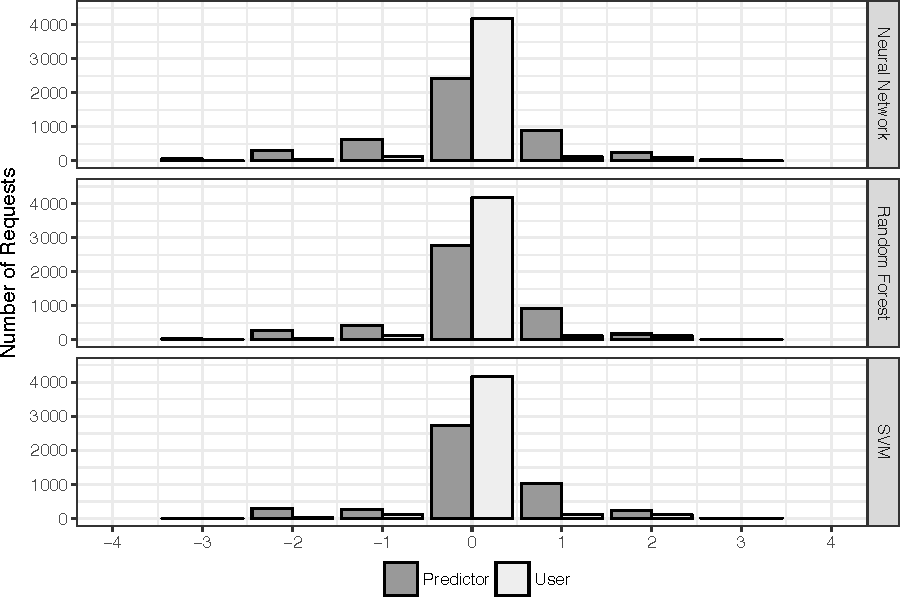
\includegraphics[scale=1]{figures/predictor_vs_user_error_magnitude.pdf}
  \caption{ML algorithms error magnitude (predictor versus user) for RQ3.}
    \label{fig:classifiers_performance_for_q3}
\end{figure*}

\begin{figure*}[!ht]
\centering
  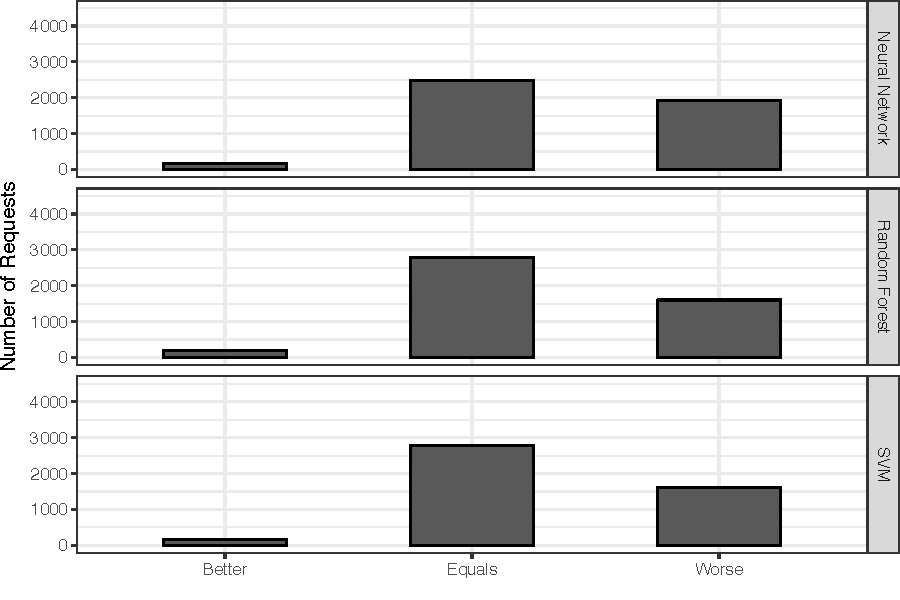
\includegraphics[scale=1]{figures/predictors_performance_compared_user.pdf}
  \caption{ML algorithms performance compared to user for RQ4.}
    \label{fig:classifiers_performance_for_q4}
\end{figure*}

\subsection{Statistical Tests}\label{subsec:tests}
We can one observe in the previous tables that the performance of the three ML algorithms are very similar. To confirm whether they are really similar, we have evaluated their F-measure performances using Friedman Test\cite{Japkowicz:2011}. 
We have defined the test null hypothesis (H0) as ``the investigated algorithms have similar performance``, and to test it, we have grouped F-measure values by dataset, research question and algorithm. For each group (3 per dataset), we have calculated the p-value.    Table \ref{tab:friedman_tests_results} shows the null hypothesis(H0) can be accepted (p$-$value $>=$ 0.05) to the most cases, confirming that the investigated algorithms are similar\cite{Demsar:2006}. 

\begin{table}[!ht]
	\renewcommand{\arraystretch}{1.8}
	\caption{Friedman tests results over F-measure.}
	\label{tab:friedman_tests_results}
	\centering
	\begin{tabular}{l|c|c|c|}
		\cline{2-4}
		
		& Question & P-value & H0\\
		\cline{1-4}
% Neural Network		
%		\multicolumn{5}{ |c| }{Neural Network}\\
%		\cline{1-5} 
        \multicolumn{1}{ |c| }{\multirow{3}{*}{\rotatebox[origin=c]{90}{\scriptsize{Cassandra}}}} & Q1 & 0.135335283 & Accepted\\
		\cline{2-4}
		\multicolumn{1}{ |c| }{} & Q2 & 0.096971968 & Accepted\\
		\cline{2-4}
        \multicolumn{1}{ |c| }{} & Q3 & 0.055637998 & Accepted\\
		\hline
		\multicolumn{1}{ |c| }{\multirow{3}{*}{\rotatebox[origin=c]{90}{\scriptsize{Hadoop}}}} & Q1 & 0.223130160 & Accepted\\
		\cline{2-4}
		\multicolumn{1}{ |c| }{} & Q2 & 0.096971968 & Accepted\\
		\cline{2-4}
		\multicolumn{1}{ |c| }{} & Q3 & 0.006737947 & Reject\\
		\hline
		\multicolumn{1}{ |c| }{\multirow{3}{*}{\rotatebox[origin=c]{90}{\scriptsize{Spark}}}} 		
		& Q1 & 0.223130160 & Accepted\\
		\cline{2-4}
		\multicolumn{1}{ |c| }{} & Q2 & 0.096971968 & Accepted\\
        \cline{2-4}
		\multicolumn{1}{ |c| }{} & Q3 & 0.040762204 & Reject\\
%		\cline{1-5} 
%		\multicolumn{1}{ |c| }{} & Average & 0.7988197 & 0.7057988 & 0.7404609\\
		\hline
	\end{tabular}
\end{table}

\subsection{Discussion}\label{subsec:discussion}

Table \ref{tab:performance_summary_literature} summarizes results related to CR severity level prediction reported in the literature and those generated during our experiments. We can observe that our results are better than others \cite{Lamkanfi2010, ValdiviaGarcia2014} to address RQ1 and RQ2. we can also note that our results are better than \cite{Tian2012} and worse than \cite{Menzies2008} to address RQ3. Notice that in many cases datasets and algorithms are different. 
\begin{table}[!h]
  \centering
  \renewcommand{\arraystretch}{1.7}
  \caption{ML algorithms performance summary (cells with a pair of numbers indicate range of variation).}
    \begin{tabular}{|c|p{2.1cm}|p{1.3cm}|c|p{1.8cm}|}
\cline{2-5}    \multicolumn{1}{r|}{} & \multicolumn{1}{c|}{Research Question} & \multicolumn{1}{c|}{Project} & F-measure & \multicolumn{1}{c|}{Algorithm} \\
    \hline
    \multirow{5}[10]{*}{\begin{turn}{88}\scriptsize{Menzies\cite{Menzies2008}}\end{turn}} & \multicolumn{1}{r|}{\multirow{5}[10]{2.1cm}{Is the bug report blocker, critical, major, minor or trivial?}} & PitsA & 14.0-17.0 & Ripper \\
\cline{3-5}          &       & PitsB & 42.0-90.0 & Ripper \\
\cline{3-5}          &       & PitsC & 53.0-92.0 & Ripper \\
\cline{3-5}          &       & PitsD & 87.0-99.0 & Ripper \\
\cline{3-5}          &       & PitsE & 8.0-88.0 & Ripper \\
    \hline
    \multirow{3}[6]{*}{\begin{turn}{88} $\quad$\scriptsize{Lamkanfi\cite{Lamkanfi2010}}\end{turn}} & \multicolumn{1}{r|}{\multirow{3}[6]{2.1cm}{Is the bug report severe or non-severe?}} & Mozilla & 65.9-71.7 & Naive Bayes \\
\cline{3-5}          &       & Eclipse & 62.5-65.5 & Naive Bayes \\
\cline{3-5}          &       & GNOME & 72.7-78.5 & Naive Bayes \\
    \hline
    \multirow{6}[12]{*}{\begin{turn}{88}\scriptsize{Valdivia\cite{ValdiviaGarcia2014}}\end{turn}} & \multicolumn{1}{r|}{\multirow{6}[12]{2.1cm}{Is the bug report blocking or non-blocking?}} & Chrominum & 15.3  & Decision Tree \\
\cline{3-5}          &       & Eclipse & 15.4  & Decision Tree \\
\cline{3-5}          &       & FreeDesktop & 31.9  & Decision Tree \\
\cline{3-5}          &       & Mozilla & 42.1  & Decision Tree \\
\cline{3-5}          &       & Netbeans & 21.1  & Decision Tree \\
\cline{3-5}          &       & Netbeans & 25.6  & Decision Tree \\
    \hline
    \multirow{3}[6]{*}{\begin{turn}{88}\scriptsize{Tian\cite{Tian2012}}\end{turn}} & \multicolumn{1}{r|}{\multirow{3}[6]{2.1cm}{Is the bug report blocker, critical, major, minor or trivial?}} & OpenOffice & 12.3-74.0 & INSPect \\
\cline{3-5}          &       & Mozilla & 13.9-65.3 & INSPect \\
\cline{3-5}          &       & Eclipse & 8.6-58.6 & INSPect \\
    \hline
    \multirow{9}[18]{*}{\begin{turn}{88}\scriptsize{Ours}\end{turn}} & \multicolumn{1}{r|}{\multirow{3}[6]{2.1cm}{Will the CR severity level change?}} & Cassandra & 65.50-97.88 & Random Forest \\
\cline{3-5}          &       & Hadoop & 53.16-97.09 & Random Forest \\
\cline{3-5}          &       & Spark & 64.15-94.87 & Random Forest \\
\cline{2-5}          & \multicolumn{1}{r|}{\multirow{3}[6]{2.1cm}{Will the CR severity level increase, decrease or remain the same?\linebreak$\quad$}} & Cassandra & 42.64-97.67 & Random Forest \\
\cline{3-5}          &       & Hadoop & 18.51-97.26 & Random Forest \\
\cline{3-5}          &       & Spark & 29.90-95.35 & Random Forest \\
\cline{2-5}          & \multicolumn{1}{r|}{\multirow{3}[6]{2.1cm}{Is the bug report blocker, critical, major, minor or trivial?}} & Cassandra & 30.15-75.43 & Random Forest \\
\cline{3-5}          &       & Hadoop & 30.76-82.01 & Random Forest \\
\cline{3-5}          &       & Spark & 14.08-73.95 & Random Forest \\
    \hline
    \end{tabular}%
  \label{tab:performance_summary_literature}%
\end{table}%  





\section{Conclusions and Research Directions}\label{sec:conclusions}

A systematic mapping review provides a structure for a research report type, which enables categorizing and giving a visual summary of results that have been published in papers of a research area\cite{Petersen:2008}. This map aids to identify gaps in a research area, becoming a basis to guide new research activities\cite{Kitchenham:2007}. The current mapping review captured the current state of research on bug report severity prediction, characterized related problems and identified the main approaches employed to solve them. These objectives were reached by conducting a mapping of existing literature. In total, the review identified 27 relevant papers and analyzed them along 12 dimensions. Although these papers have made valuable contributions in bug report severity prediction, the panorama presented in this mapping review suggests that there are potential research opportunities for further improvements in this topic. Among them, the following research directions appear to be more promising:

\begin{itemize}
  \item There is an apparent lack of investigation on bug report severity prediction in other relevant FLOSS such as, for example, Linux Kernel, Ubuntu Linux, and MySQL, and in others BTS, for example, Github.
  \item Often, technical users report most bugs. Thus, the influence of user experience in predicting outcomes is still overlooked.  
  \item Bug reports labeled with default severity level (often ``normal") were prevalent in the most datasets used in reviewed papers. However, they are considered unreliable\cite{Saha:2015}, and just discarding them also does not seem appropriate. Then, efforts in researching on novel approaches to handle this type of report should be considered to improve the state-of-the-art of severity prediction algorithms.
  \item Most approaches were based on unstructured text features (\textit{summary} and \textit{description}). To handle them, researchers chose to use the traditional bag-of-words approach instead of more recent text mining methods (e.g., word-embedding\cite{Guoyin:2018}) or data-driven feature engineering methods which may likely improve outcomes yielded so far.
  \item There is a clear research opportunity to investigate whether state-of-the-art ML algorithms might outperform the traditional algorithms used in all reviewed papers for bug report severity prediction. The investigation of the use of Deep learning algorithms which perform very well when classifying audio, text, and image data\cite{Goodfellow:2016} seems to be a promising research direction.
  \item Researchers should investigate more recent techniques (e.g., continuous learning\cite{Chen:2016}) to provide an approach for bug report prediction which could be employed in real-world scenarios.
  \item Many bug reports are resolved in a few days (or in a few hours)\cite{Saha:2015b}. Efforts to predict severity level for these group of bug reports do not seem very useful. Thus, an investigation to confirm this hypothesis and to determine when the severity prediction is more appropriate in bug report lifecycle is of critical importance.
\end{itemize}

%\section*{Acknowledgment}
(omitted for double-blind reviewing). 

\bibliographystyle{IEEEtran}
\bibliography{references}

\end{document}


